\documentclass[11pt,a4paper]{article}
\usepackage[margin=1in]{geometry}
\usepackage[T1]{fontenc}
\usepackage[utf8]{inputenc}
\usepackage{lmodern}
\usepackage{microtype}
\usepackage{amsthm,amsmath,amssymb,amsfonts}
\usepackage{mathtools}
\usepackage{booktabs}
\usepackage{graphicx}
\usepackage{tikz}
\usepackage{subcaption}
\usepackage{ifthen}
\usetikzlibrary{arrows,decorations.pathmorphing,decorations.pathreplacing,backgrounds,positioning,fit,matrix,shapes,calc,mindmap}
\usepackage[colorlinks,urlcolor=blue!50!black,linkcolor=blue!50!black,citecolor=green!40!black]{hyperref}
\usepackage{cleveref}
\usepackage{etoolbox}

\definecolor{myred}{rgb}{0.75,0,0}
\definecolor{myblue}{rgb}{0,0,0.72}
\definecolor{mygreen}{rgb}{0,0.5,0}
\definecolor{mysolutioncolor}{rgb}{0.72,0.52,0}
\definecolor{mygray}{rgb}{0.55,0.55,0.55}

\newtheorem{theorem}{Theorem}
\newcounter{theoremanchor}
\AtBeginEnvironment{theorem}{\stepcounter{theoremanchor}}
\providecommand{\theHtheorem}{}
\renewcommand{\theHtheorem}{\arabic{theoremanchor}}
\newtheorem{lemma}{Lemma}
\newtheorem*{supportingtheorem}{Theorem}
\newtheorem{corollary}{Corollary}
\newtheorem{observation}{Observation}
\theoremstyle{definition}
\newtheorem{definition}{Definition}
\crefname{observation}{Observation}{Observations}
\Crefname{observation}{Observation}{Observations}

\newcommand{\doi}[1]{DOI: \href{https://doi.org/#1}{\nolinkurl{#1}}}
\newcommand{\threefield}[3]{$#1\mid#2\mid#3$}
\newcommand{\rep}{\mathrm{rep}}
\newcommand{\q}{m}
\newcommand{\EQUIJIT}{\threefield{1}{\rep}{\min_j \sum_i Z_{i,j}}}
\newcommand{\OPEQUIJIT}{\threefield{1}{\rep, d_{i,j}=d_j}{\min_j \sum_i Z_{i,j}}}
\newcommand{\DDEQUIJIT}{\threefield{1}{\rep, p_{i,j}=p_j}{\min_j \sum_i Z_{i,j}}}
\newcommand{\UEQUIJIT}{\threefield{1}{\rep, p_{i,j}=1}{\min_j \sum_i Z_{i,j}}}
\newcommand{\SDEQUIJIT}{\threefield{1}{\rep, d_{i,j}=d_j, p_{i,j}=p_j}{\min_j \sum_i Z_{i,j}}}
\newcommand{\WEQUIJIT}{\threefield{1}{k_j,\rep}{\min_j \sum_i Z_{i,j}}}
\newcommand{\MCIS}{\textsc{Multicoloured Independent Set}}
\newcommand{\MCC}{\textsc{Multicoloured Clique}}
\newcommand{\SAT}{[2,3]-\textsc{bounded 3-SAT}}
\newcommand{\bigO}{O}
\newcommand{\NP}{\textnormal{\textsf{NP}}}

\title{Fair Repetitive Interval Scheduling}
\author{Yuval Itzhaki \and Claude}
\date{}

\begin{document}
\maketitle

\begin{abstract}
This note presents the formalization of the paper of Heeger, Hermelin, Itzhaki, Molter and
Shabtay~\cite{HHIMS}:~$n$ clients each submit one just-in-time job on every one of~$m$
days, and a schedule is \emph{fair} if every client is served on at least~$k$ of the days.
A job with processing time~$p$ and due date~$d$ occupies exactly the interval~$(d-p,d]$.
The paper gives a complete dichotomy of the problem's complexity in the fairness parameter~$k$, settles the two natural restrictions to day-independent processing times and
day-independent due dates, and determines the complexity with respect to the treewidth of
the daily conflict structure and the number of clients. The development proves the scheduling results and supporting algorithmic statements in Lean. The construction gives inactive clients disjoint slots
inside the dummy client's interval, preserving the conflict graph needed for the
treewidth bound. A reduction from \SAT\ establishes the required hardness of
\textsc{Multicoloured Independent Set} on regular instances. This note presents the
statements in the notation of~\cite{HHIMS}, with links to their Lean counterparts.
For completeness, the supporting results of Bodlaender and Kloks on finding nice tree
decompositions of bounded width are also formalized. This general graph algorithm
development goes beyond the scheduling scope of the project and supplies the
decompositions used by its scheduling algorithm.
\end{abstract}

\section{Introduction}

% lax begin Lax117284.Scheduling
\begin{definition}
\label{def:equijit}
$n$ clients and~$m$ days. Client~$j$'s job on day~$i$ has a processing time~$p_{i,j}\ge1$ and a due date~$d_{i,j}\ge p_{i,j}$, and occupies exactly the interval~$(d_{i,j}-p_{i,j},\,d_{i,j}]$. Two jobs of the same day \emph{conflict} if their intervals
intersect. One machine is available on each day; a \emph{schedule} selects, for every day,
a set of clients whose jobs that day are pairwise non-conflicting (the rest are rejected
that day). Writing~$Z_{i,j}$ for the indicator that client~$j$ is served on day~$i$, a
schedule is \emph{$k$-fair} if~$\sum_iZ_{i,j}\ge k$ for every client~$j$. Given~$k$, is
there a~$k$-fair schedule?
\end{definition}
% lax end

% lax begin lax-808846
Running times below are stated on the word RAM. A program is a fixed list of instructions
operating on words of~$w$ bits, and its running time is the number of instructions it
executes on an input word, under the word-length and workspace conditions stated in the linked concepts.
% lax end

\cite{HHIMS} gives a complete answer in the fairness parameter alone:

% lax begin Lax117284.Theorem1
\setcounter{theorem}{0}
\begin{theorem}
\label{thm:1}
For~$0\le k\le m$, \EQUIJIT\ is solvable in polynomial time when~$k\in\{0,m-1,m\}$. It is NP-hard for every fixed pair~$(m,k)$ with~$0<k<m-1$.
\end{theorem}
% lax end
and then studies two restrictions, \emph{day-independent processing times}
($p_{i,j}=p_j$) and \emph{day-independent due dates} ($d_{i,j}=d_j$), and two structural
parameters of the \emph{overall conflict graph}~$G$, the graph on the clients in which two
are adjacent exactly when some day's jobs of theirs conflict.

\section{Preliminaries}

% lax begin Lax117284.ConflictGraph
A day's conflict graph is an interval graph, and a schedule is feasible on a day exactly
when its set of clients is independent in that day's graph. The \emph{overall conflict
graph}~$G$ is the union, over all days, of the daily conflict graphs; its \emph{treewidth}~$\tau$ is the structural parameter of \Cref{sec:fpt}.
% lax end
% lax begin Lax117284.Bodlaender
A tree decomposition of a graph is a tree of bags of vertices, every vertex and every edge
in some bag, the bags containing a fixed vertex forming a connected subtree; its width is
the largest bag size minus one, and the treewidth of a graph is the least width of a tree
decomposition of it. Given a width bound~$w$, Bodlaender's algorithm finds a tree
decomposition of width at most~$w$ or determines that none exists, in
time~$2^{\bigO(w^3)}\cdot\mathrm{poly}$.
% lax end
An algorithm is \emph{fixed-parameter tractable} (FPT) for a parameter~$\kappa$ if it runs
in~$f(\kappa)\cdot N^{\bigO(1)}$ time for some computable~$f$, where~$N$
is the binary input size. We use the shared fixed-parameter time definition
from the archive; the structural parameter~$m+\tau$ need not itself be
computed in polynomial time.

\section{The Fairness Parameter}
\label{sec:k}

% lax begin Lax117284.Theorem7
\setcounter{theorem}{6}
\begin{theorem}
\label{thm:7}
\EQUIJIT\ is NP-hard already at~$k=1$,~$m=3$, and with every job's processing time equal.
\end{theorem}
% lax end
The reduction is from \SAT. Given a formula with~$\ell$ two-literal and~$q$ three-literal
clauses over~$n$ variables, every processing time is~$2$, so two jobs of a day conflict
exactly when their due dates differ by at most one, and the whole construction places due
dates on a line, three times over. It uses three \emph{dummy} clients, two clients~$x_v^1,x_v^0$
per variable, and one client per literal occurrence, with due dates chosen so that a~$1$-fair schedule of the three days exists exactly when the formula is satisfiable.

% lax begin Lax117284.Corollary8
\setcounter{corollary}{7}
\begin{corollary}
\label{cor:8}
\EQUIJIT\ is NP-hard for every~$m\ge3$ and~$0<k<m-1$.
\end{corollary}
% lax end
Two reductions lift \Cref{thm:7} to every such pair: adding one conflict-free day raises
both~$m$ and the attainable fairness by one, taking~$(m,k)$ to~$(m+1,k+1)$; and adding one
day together with one new client that conflicts with every job of every old day, and whose
own job occupies the new day alone, forces the new client onto the new day in any~$1$-fair
schedule, taking~$(m,1)$ to~$(m+1,1)$. Chaining these from~$(3,1)$ reaches every~$(m,k)$ with~$m\ge3$ and~$0<k<m-1$.

% lax begin Lax117284.Theorem9
\setcounter{theorem}{8}
\begin{theorem}
\label{thm:9}
\EQUIJIT\ is solvable in polynomial time when~$k=m-1$.
\end{theorem}
% lax end
A variable~$x_{i,j}$ per day and client; a \emph{conflict clause}~$(\lnot x_{i,j_1}\lor\lnot x_{i,j_2})$ for every conflicting pair on a day, and a
\emph{validation clause}~$(x_{i_1,j}\lor x_{i_2,j})$ for every client and every two days
(forbidding two rejections) give a 2-CNF formula satisfiable exactly when a~$(m-1)$-fair
schedule exists. The formalization uses its verified polynomial-time 2-SAT algorithm.

\Cref{thm:1} follows from \Cref{cor:8} and \Cref{thm:9}, together with the trivial cases~$k=0$ and~$k=m$.

\section{Day-Independent Processing Times and Due Dates}
\label{sec:dayindep}

% lax begin Lax117284.Theorem2
\setcounter{theorem}{1}
\begin{theorem}[Hardness]
\label{thm:2hard}
\DDEQUIJIT\ is NP-hard.
\end{theorem}
% lax end
\Cref{thm:7}'s reduction already produces instances of equal, hence day-independent,
processing times, so \Cref{cor:8}'s lift carries this hardness to every~$m\ge3,\,0<k<m-1$.

% lax begin Lax117284.Theorem10
\setcounter{theorem}{9}
\begin{theorem}
\label{thm:10}
With unit processing times, two jobs of a day conflict exactly when their due dates agree.
An instance with~$k\le m$ admits a~$k$-fair schedule if and only if the bipartite graph
with a \emph{job} vertex~$v_{i,j}$ per day and client, a \emph{due-date} vertex~$u_{i,t}$
per day and distinct due date, and~$m-k$ \emph{rejection} vertices~$w_{1,j},\dots,w_{m-k,j}$
per client, joining~$v_{i,j}$ to~$u_{i,d_{i,j}}$ and to every rejection vertex of
client~$j$, has a matching saturating every job vertex.
\end{theorem}
% lax end

% Adapted from the thesis chapter on fair repetitive interval scheduling.
\begin{figure}
    \centering
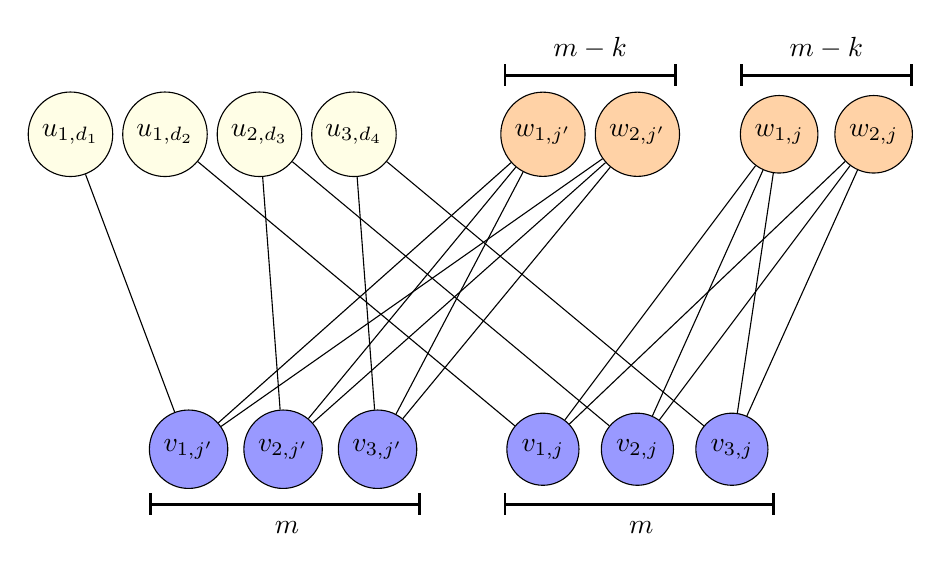
\begin{tikzpicture}

  \node[] at (1.2*1+3.5+1.75-4.5, -1.) {$\q$};
   \draw[line width=1, |-|]
  (1.2+3.5-4.5, -.7) -- (1.2*2+5.75-4.5, -.7) node[anchor=north] {};
  \foreach \i in {1,...,3} {
    \node[draw, circle, fill=blue!40] (A\i) at (\i*1.2-.5, 0) {$v_{\i,j'}$};
  }

  \node[] at (1.2*1+3.5+1.75, -1.) {$\q$};
   \draw[line width=1, |-|]
  (1.2+3.5, -.7) -- (1.2*2+5.75, -.7) node[anchor=north] {};
 
  \foreach \i in {1,...,3} {
    \node[draw, circle, fill=blue!40] (C\i) at (\i*1.2+4, 0) {$v_{\i,j}$};
  }
  
  \node[] at (1.2*1+4.6, 5.1) {$\q-k$};
   \draw[line width=1, |-|]
  (1.2+3.5, 4.75) -- (1.2*2+4.5, 4.75) node[anchor=north] {};
  \foreach \i in {1,...,2} {
    \node[draw, circle, fill=orange!35] (B\i) at (\i*1.2+4, 4) {$w_{\i,j'}$};
  }

  \node[] at (1.2*1+7.6, 5.1) {$\q-k$};
   \draw[line width=1, |-|]
  (1.2+6.5, 4.75) -- (1.2*2+7.5, 4.75) node[anchor=north] {};
  \foreach \i in {1,...,2} {
    \node[draw, circle, fill=orange!35] (D\i) at (\i*1.2+7, 4) {$w_{\i,j}$};
  }

    \node[draw, circle, fill=yellow!10] (F1) at (1*1.2-2, 4) {$u_{1,d_1}$};
    \node[draw, circle, fill=yellow!10] (F2) at (2*1.2-2, 4) {$u_{1,d_2}$};
    \node[draw, circle, fill=yellow!10] (F3) at (3*1.2-2, 4) {$u_{2,d_3}$};
    \node[draw, circle, fill=yellow!10] (F4) at (4*1.2-2, 4) {$u_{3,d_4}$};
                

  \foreach \i in {1,...,3} {
    \foreach \j in {1,...,2} {
      \draw (A\i) -- (B\j);
      \draw (C\i) -- (D\j);
    }
  }

    \draw (A1) -- (F1);
    \draw (C1) -- (F2);

    \draw (C2) -- (F3);
    \draw (A2) -- (F3);

    \draw (C3) -- (F4);
    \draw (A3) -- (F4);
    
\end{tikzpicture}

\caption{
The construction of a bipartite graph from an instance of \UEQUIJIT\ with $\q=3$ and $k=1$, where only the relevant vertices for two clients~$j$ and~$j'$ are depicted. Clients $j$ and~$j'$ have different due dates on day 1, and the same due date on days 2 and 3. Each client has two rejection vertices, adjacent to all three of that client's job vertices.}
\label{fig:bipartiteM}%
\end{figure}


% lax begin Lax117284Proofs.Theorem2UnitP.uniform_unitP_mem_P
\setcounter{theorem}{1}
\begin{theorem}[Tractability]
\label{thm:2trac}
\UEQUIJIT\ is solved in polynomial time, by \Cref{thm:10} and a maximum bipartite matching
algorithm.
\end{theorem}
% lax end

% lax begin Lax117284.Theorem11
\setcounter{theorem}{10}
\begin{theorem}
\label{thm:11}
\OPEQUIJIT\ is NP-hard.
\end{theorem}
% lax end
Reading an instance of \threefield{R}{}{\sum_j Z_j} (unrelated machines, maximizing the
just-in-time jobs) as one of \OPEQUIJIT\ with jobs as clients and machines as days gives an
instance at~$k=1$ that is a yes-instance exactly when every job of the source can be
scheduled just in time, which is NP-hard~\cite{Sung05}.

% lax begin Lax117284.Theorem12
\setcounter{theorem}{11}
\begin{theorem}
\label{thm:12}
With day-independent due dates and a constant number~$m$ of days, \EQUIJIT\ is solved in
polynomial time.
\end{theorem}
% lax end
Ordering the clients by due date, a dynamic program carries, for each day, the time at
which its machine next frees up; serving a client on a set of days needs each of those
machines free early enough, and leaves each free from the client's due date onwards. Since
later clients have due dates at least as large, this state is exactly what the decision
about earlier clients needs to leave behind, and for constant~$m$ there are polynomially
many states.

% lax begin Lax117284.Theorem13
\setcounter{theorem}{12}
\begin{theorem}
\label{thm:13}
With both due dates and processing times day-independent, every day has the same conflict
graph~$G$, and \SDEQUIJIT\ is solvable in polynomial time, since a~$k$-fair schedule exists
exactly when~$k\cdot\chi(G)\le m$, where~$\chi(G)$ is the chromatic number of~$G$.
\end{theorem}
% lax end
A~$\chi(G)$-colouring partitions the clients into~$\chi(G)$ independent sets, scheduled in
rotation; conversely a clique of~$G$ needs one day per client per repetition, and since~$G$
is an interval graph its chromatic number equals its clique number, so the two bounds
coincide.

\section{Complexity of Structural Parameters}
\label{sec:fpt}

% lax begin Lax117284.Theorem4
\setcounter{theorem}{3}
\begin{theorem}[Bounded-Treewidth Hardness]
\label{thm:4a}
\EQUIJIT\ is NP-hard on instances whose overall conflict graph has treewidth at most~$6$, and hence under any fixed treewidth upper bound of at least~$6$.
\end{theorem}
% lax end
The reduction is in two steps, a per-client generalization at treewidth~$4$
(\Cref{lem:14}), then a uniform-parameter reduction raising the treewidth by at most~$2$
(\Cref{lem:15}).

\subsection{Hardness at Bounded Treewidth}

% lax begin Lax117284.MulticolouredIndepSet
\MCIS\ asks, given an~$\ell$-partite graph~$G=(V_1\cup\dots\cup V_\ell,E)$, is there a choice of
one vertex per class with no two chosen vertices adjacent? It is NP-hard.

\begin{quote}
\textbf{Regular Source Instances.} Lemma 14's reduction uses~$G$ in \emph{normal form}:~$r$-regular with~$r\ge1$, every class of~$n\ge4$ vertices, and~$|E|$ even.
The formalization proves \MCIS\ NP-hard on these instances directly, by a
reduction from \SAT~\cite{Tovey84}: the occurrence graph of a formula (one vertex per
clause position) is made regular by five uniform \emph{ports} per
position, each a seven-vertex gadget whose independence number is fixed whether or not its
port is used, and the resulting graph is then replaced by a disjoint union of copies of
itself, with the colour classes defined by the construction, which fixes the parity of~$|E|$ without
touching~$r$-regularity or the existence of a multicoloured independent set.
\end{quote}
% lax end

% lax begin Lax117284.Lemma14
\setcounter{lemma}{13}
\begin{lemma}
\label{lem:14}
\WEQUIJIT, the variant of \EQUIJIT\ with one fairness parameter~$k_j$ per client, is NP-hard even when the overall conflict graph has
treewidth at most~$4$.
\end{lemma}
From a normal-form \MCIS\ instance~$G$ we build~$\ell(n+1)+|E|$ days (for every colour~$n$
\emph{vertex days} and one \emph{validation day}, and one \emph{edge day} per edge) and
the following clients. A \emph{vertex client}~$c_v$ ($k_{c_v}=1$) per vertex, a \emph{selection client}~$c_i$ ($k_{c_i}=1$) per colour, two \emph{edge clients}~$c_{v,u},c_{u,v}$ ($k=1$) per
edge, two \emph{interaction clients}~$c^+,c^-$ ($k^+=k^-=|E|/2$), and a \emph{dummy client}~$c_0$ with~$k_0$ equal to the number of days. On every day, only a handful of clients take
part in that day's gadget, and~$c_0$'s job, the longest of the day, \emph{blocks} every
other client not named in the gadget, forcing it to be rejected that day.

\begin{quote}
\textbf{Blocking Inactive Jobs.} Giving all inactive clients the same interval would
make them pairwise adjacent in the conflict graph. To preserve the treewidth bound,
each inactive client instead occupies a separate unit-length slot inside~$c_0$'s interval:
numbering the clients other than~$c_0$ by a
bijection~$\pi$ with~$\{1,\dots,N\}$,~$c_0$'s job has processing time~$N$ and due date~$r+N$
(say, on a vertex day), and a blocked client~$c$'s job is the single time unit at offset~$\pi(c)$, due date~$r+\pi(c)$. Every blocked client still conflicts with~$c_0$, since its slot
lies inside~$c_0$'s interval, but no two blocked clients conflict with each other, since
their slots are disjoint. \Cref{fig:vsg,fig:edgeday} show the resulting gadgets.
The formalization proves the stated tree decomposition for this construction.
\end{quote}
% lax end

% copied from the thesis chapter on fairness (content/fairness/fairness.tex, lines 504-766)
\begin{figure}[t]
\centering
\scalebox{0.72}{\begin{minipage}{\textwidth}%
\begin{subfigure}{0.4\textwidth}
\begin{center}
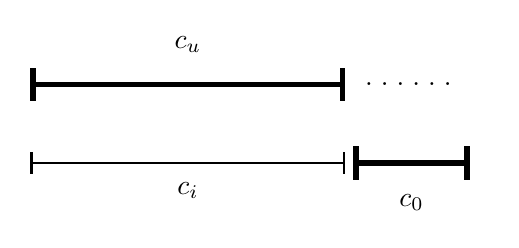
\begin{tikzpicture}
  \draw[line width=2, |-|]
  ({0.5}, 2.5) -- ({4.5}, 2.5) node[anchor=north west] {};
  \node at ({2.5}, 3) {$c_u$};
  \draw[line width=1, |-|]
  ({0.5}, 1.5) -- ({4.5}, 1.5) node[anchor=north west] {};
  \node at ({2.5},1.15) {$c_i$};
  \draw[line width=2, |-|]
  ({4.6}, 1.5) -- ({6.08}, 1.5) node[anchor=north west] {};
  \node at ({5.34}, 1.) {$c_0$};
  \node at ({5.3}, 3.) {};% {$c\in X$};
  \foreach \x in
    {
        1,2,3,4,5,6
    }
    {
        \node at ({4.6+\x*0.2}, 2.5) {$.$};
    }
\end{tikzpicture}
\caption{The vertex-selection day for $u\in V_i$, where $u \notin I$.
}
\end{center}
\end{subfigure}
\hspace{1cm}
\begin{subfigure}{0.4\textwidth}
\begin{center}
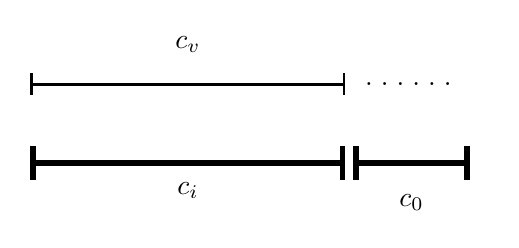
\begin{tikzpicture}
  \draw[line width=1, |-|]
  ({0.5}, 2.5) -- ({4.5}, 2.5) node[anchor=north west] {};
  \node at ({2.5}, 3) {$c_v$};
  \draw[line width=2, |-|]
  ({0.5}, 1.5) -- ({4.5}, 1.5) node[anchor=north west] {};
  \node at ({2.5},1.15) {$c_i$};
  \draw[line width=2, |-|]
  ({4.6}, 1.5) -- ({6.08}, 1.5) node[anchor=north west] {};
  \node at ({5.34}, 1.) {$c_0$};
  \node at ({5.3}, 3.) {};% {$c\in X$};
  \foreach \x in
    {
        1,2,3,4,5,6
    }
    {
        \node at ({4.6+\x*0.2}, 2.5) {$.$};
    }
\end{tikzpicture}
\caption{The vertex-selection day for $v\in V_i$, where $v \in I$.
}
\end{center}
\end{subfigure}

\vspace{0.5cm}

\begin{subfigure}{\textwidth}
\begin{center}
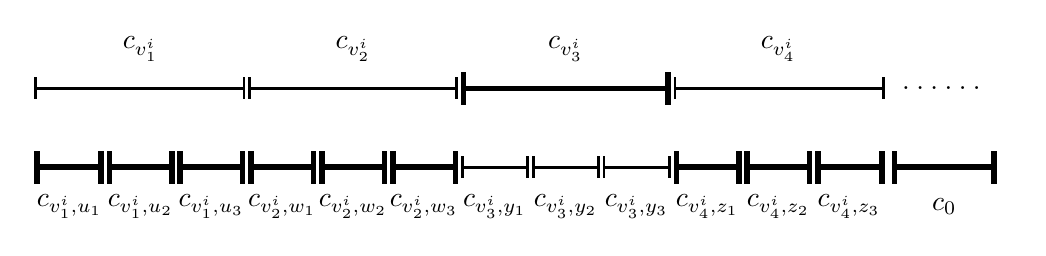
\begin{tikzpicture}[xscale=0.9]

  \draw[line width=1, |-|]
  ({0.5}, 2.5) -- ({3.48}, 2.5) node[anchor=north west] {};
  \node at ({2.}, 3) {$c_{v_1^i}$};
  \draw[line width=1, |-|]
  ({3.52}, 2.5) -- ({6.48}, 2.5) node[anchor=north west] {};
  \node at ({5.}, 3) {$c_{v_2^i}$};
  \draw[line width=2, |-|]
  ({6.52}, 2.5) -- ({9.48}, 2.5) node[anchor=north west] {};
  \node at ({8}, 3) {$c_{v_3^i}$};
  \draw[line width=1, |-|] ({9.52}, 2.5) -- ({12.5}, 2.5) node[anchor=north west] {};
  \node at ({11.}, 3) {$c_{v_4^i}$};

  \draw[line width=2, |-|]
  ({0.5}, 1.5) -- ({1.48}, 1.5) node[anchor=north west] {};
  \node at (1, 1.) {$c_{v_1^i,u_1}$};
  \draw[line width=2, |-|]
  ({1.52}, 1.5) -- ({2.48}, 1.5) node[anchor=north west] {};
  \node at (2, 1.) {$c_{v_1^i,u_2}$};
  \draw[line width=2, |-|]
  ({2.52}, 1.5) -- ({3.48}, 1.5) node[anchor=north west] {};
  \node at (3, 1.) {$c_{v_1^i,u_3}$};

  \draw[line width=2, |-|]
  ({3.52}, 1.5) -- ({4.48}, 1.5) node[anchor=north west] {};
  \node at (4, 1.) {$c_{v_2^i,w_1}$};
  \draw[line width=2, |-|]
  ({4.52}, 1.5) -- ({5.48}, 1.5) node[anchor=north west] {};
  \node at (5, 1.) {$c_{v_2^i,w_2}$};
  \draw[line width=2, |-|]
  ({5.52}, 1.5) -- ({6.48}, 1.5) node[anchor=north west] {};
  \node at (6, 1.) {$c_{v_2^i,w_3}$};

  \draw[line width=1, |-|]
  ({6.52}, 1.5) -- ({7.48}, 1.5) node[anchor=north west] {};
  \node at (7, 1.) {$c_{v_3^i,y_1}$};
  \draw[line width=1, |-|]
  ({7.52}, 1.5) -- ({8.48}, 1.5) node[anchor=north west] {};
  \node at (8, 1.) {$c_{v_3^i,y_2}$};
  \draw[line width=1, |-|]
  ({8.52}, 1.5) -- ({9.48}, 1.5) node[anchor=north west] {};
  \node at (9, 1.) {{$c_{v_3^i,y_3}$}};

  \draw[line width=2, |-|]
  ({9.52}, 1.5) -- ({10.48}, 1.5) node[anchor=north west] {};
  \node at (10, 1.) {{$c_{v_4^i,z_1}$}};
  \draw[line width=2, |-|]
  ({10.52}, 1.5) -- ({11.48}, 1.5) node[anchor=north west] {};
  \node at (11, 1.) {$c_{v_4^i,z_2}$};
  \draw[line width=2, |-|]
  ({11.52}, 1.5) -- ({12.5}, 1.5) node[anchor=north west] {};
  \node at (12, 1.) {$c_{v_4^i,z_3}$};

  \draw[line width=2, |-|]
  ({12.6}, 1.5) -- ({14.08}, 1.5) node[anchor=north west] {};
  \node at ({13.34}, 1.) {$c_0$};
  \node at ({13.3}, 3.) {};% {$c\in X$};
  \foreach \x in
    {
        1,2,3,4,5,6
    }
    {
        \node at ({12.6+\x*0.2}, 2.5) {$.$};
    }
\end{tikzpicture}
\caption{The $i$-th validation day where $v^i_3\in I$.}
\end{center}
\end{subfigure}

    

    
  
  
  
  

\end{minipage}}
\caption{An example of schedules on the vertex selection days and the validation days given a multicoloured independent set $I$. We mark in \textbf{bold} the jobs which are scheduled; the jobs not appearing in the gadget are shown schematically by dots, are pairwise disjoint and are all contained in the job of client $c_0$. }
\label{fig:vsg}%
\end{figure}


% copied from the thesis chapter on fairness (content/fairness/fairness.tex, lines 779-1003)
\begin{figure}[!htbp]
  \begin{center}
      
    \begin{subfigure}[t]{0.3\textwidth}
        \begin{center}
            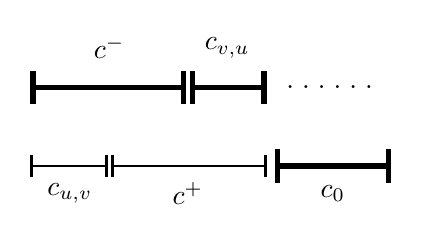
\begin{tikzpicture}

  \draw[line width=2, |-|]
  ({0.5}, 2.5) -- ({2.48}, 2.5) node[anchor=north west] {};
  \node at ({1.5}, 3) {$c^-$};
  \draw[line width=1, |-|]
  ({1.52}, 1.5) -- ({3.5}, 1.5) node[anchor=north west] {};
  \node at ({2.5},1.15) {$c^+$};
  
  \draw[line width=1, |-|]
  ({.5}, 1.5) -- ({1.48}, 1.5) node[anchor=north west] {};
  \node at ({1.},1.15) {$c_{u,v}$};
  \draw[line width=2, |-|]
  ({2.52}, 2.5) -- ({3.5}, 2.5) node[anchor=north west] {};
  \node at ({3.},3) {$c_{v,u}$};

  % the job of $c_0$, containing the jobs of the clients not mentioned above
  \draw[line width=2, |-|]
  ({3.6}, 1.5) -- ({5.08}, 1.5) node[anchor=north west] {};
  \node at ({4.34}, 1.15) {$c_0$};
  \node at ({4.3}, 3.) {}; % {$c$};
  \foreach \x in
    {
        1,2,3,4,5,6
    }
    {
        \node at ({3.6+\x*0.2}, 2.5) {$.$};
    }
  
            \end{tikzpicture}
        \end{center}
        \caption{$v\in I , u \notin I$.}
        \end{subfigure}
        \hspace{.3cm}
           \begin{subfigure}[t]{0.3\textwidth}
        \begin{center}
            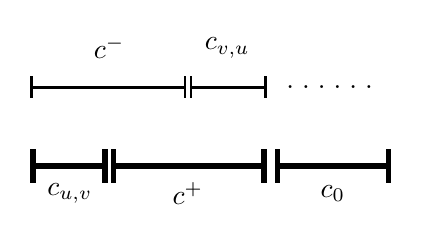
\begin{tikzpicture}

  \draw[line width=1, |-|]
  ({0.5}, 2.5) -- ({2.48}, 2.5) node[anchor=north west] {};
  \node at ({1.5}, 3) {$c^-$};
  \draw[line width=2, |-|]
  ({1.52}, 1.5) -- ({3.5}, 1.5) node[anchor=north west] {};
  \node at ({2.5},1.15) {$c^+$};
  
  \draw[line width=2, |-|]
  ({.5}, 1.5) -- ({1.48}, 1.5) node[anchor=north west] {};
  \node at ({1.},1.15) {$c_{u,v}$};
  \draw[line width=1, |-|]
  ({2.52}, 2.5) -- ({3.5}, 2.5) node[anchor=north west] {};
  \node at ({3.},3) {$c_{v,u}$};

  % the job of $c_0$, containing the jobs of the clients not mentioned above
  \draw[line width=2, |-|]
  ({3.6}, 1.5) -- ({5.08}, 1.5) node[anchor=north west] {};
  \node at ({4.34}, 1.15) {$c_0$};
  \node at ({4.3}, 3.) {}; % {$c$};
  \foreach \x in
    {
        1,2,3,4,5,6
    }
    {
        \node at ({3.6+\x*0.2}, 2.5) {$.$};
    }
  
            \end{tikzpicture}
        \end{center}
        \caption{$ v \notin I, u\in I$.}
        \end{subfigure}      
        \hspace{.3cm}
        \begin{subfigure}[t]{0.3\textwidth}
        \begin{center}
            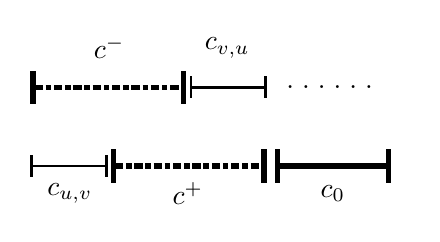
\begin{tikzpicture}

  \draw[line width=2, densely dash dot, |-|]
  ({0.5}, 2.5) -- ({2.48}, 2.5) node[anchor=north west] {};
  \node at ({1.5}, 3) {$c^-$};
  \draw[line width=2, densely dash dot, |-|]
  ({1.52}, 1.5) -- ({3.5}, 1.5) node[anchor=north west] {};
  \node at ({2.5},1.15) {$c^+$};
  
  \draw[line width=1, |-|]
  ({.5}, 1.5) -- ({1.48}, 1.5) node[anchor=north west] {};
  \node at ({1.},1.15) {$c_{u,v}$};
  \draw[line width=1, |-|]
  ({2.52}, 2.5) -- ({3.5}, 2.5) node[anchor=north west] {};
  \node at ({3.},3) {$c_{v,u}$};

  % the job of $c_0$, containing the jobs of the clients not mentioned above
  \draw[line width=2, |-|]
  ({3.6}, 1.5) -- ({5.08}, 1.5) node[anchor=north west] {};
  \node at ({4.34}, 1.15) {$c_0$};
  \node at ({4.3}, 3.) {}; % {$c$};
  \foreach \x in
    {
        1,2,3,4,5,6
    }
    {
        \node at ({3.6+\x*0.2}, 2.5) {$.$};
    }
  
\end{tikzpicture}
\end{center}
\caption{$u,v \notin I$: schedule either $c^+$ or\ $c^-$ such that $c^+$ and $c^-$ are satisfied. }
\end{subfigure}
  \end{center}
%   \begin{center}
      
%     \begin{subfigure}[t]{0.3\textwidth}
%         \begin{center}
%             \begin{tikzpicture}

%     \draw[line width=2, |-|]
%   ({0.48}, 1.5) -- ({-1.}, 1.5) node[anchor=north west] {};
%   \node at (({-.25}, 1.15) {$c_0$};
%   \node at ({-0.25}, 3.) {}; % {$c$};
%   \foreach \x in
%     {
%         1,2,3,4,5,6
%     }
%     {
%         \node at ({-1+\x*0.2}, 2.5) {$.$};
%     }
  
  
%   \draw[line width=2, |-|]
%   ({0.5}, 2.5) -- ({2.48}, 2.5) node[anchor=north west] {};
%   \node at (({1.5}, 3) {$c^-$};
%   \draw[line width=1, |-|]
%   ({1.52}, 1.5) -- ({3.5}, 1.5) node[anchor=north west] {};
%   \node at ({2.5},1.15) {$c^+$};
  
%   \draw[line width=1, |-|]
%   ({.5}, 1.5) -- ({1.48}, 1.5) node[anchor=north west] {};
%   \node at ({1.},1.15) {$c_{u,v}$};
%   \draw[line width=2, |-|]
%   ({2.52}, 2.5) -- ({3.5}, 2.5) node[anchor=north west] {};
%   \node at ({3.},3) {$c_{v,u}$};
  
%             \end{tikzpicture}
%         \end{center}
%         \caption{$v\in I , u \notin I$.}
%         \end{subfigure}
%         \hspace{.3cm}
%            \begin{subfigure}[t]{0.3\textwidth}
%         \begin{center}
%             \begin{tikzpicture}

%              \draw[line width=2, |-|]
%   ({0.48}, 1.5) -- ({-1.}, 1.5) node[anchor=north west] {};
%   \node at (({-.25}, 1.15) {$c_0$};
%   \node at ({-0.25}, 3.) {}; % {$c$};
%   \foreach \x in
%     {
%         1,2,3,4,5,6
%     }
%     {
%         \node at ({-1+\x*0.2}, 2.5) {$.$};
%     }
                
%   \draw[line width=1, |-|]
%   ({0.5}, 2.5) -- ({2.48}, 2.5) node[anchor=north west] {};
%   \node at (({1.5}, 3) {$c^-$};
%   \draw[line width=2, |-|]
%   ({1.52}, 1.5) -- ({3.5}, 1.5) node[anchor=north west] {};
%   \node at ({2.5},1.15) {$c^+$};
  
%   \draw[line width=2, |-|]
%   ({.5}, 1.5) -- ({1.48}, 1.5) node[anchor=north west] {};
%   \node at ({1.},1.15) {$c_{u,v}$};
%   \draw[line width=1, |-|]
%   ({2.52}, 2.5) -- ({3.5}, 2.5) node[anchor=north west] {};
%   \node at ({3.},3) {$c_{v,u}$};
  
%             \end{tikzpicture}
%         \end{center}
%         \caption{$ v \notin I, u\in I$.}
%         \end{subfigure}      
%         \hspace{.3cm}
%         \begin{subfigure}[t]{0.3\textwidth}
%         \begin{center}
%             \begin{tikzpicture}

%              \draw[line width=2, |-|]
%   ({0.48}, 1.5) -- ({-1.}, 1.5) node[anchor=north west] {};
%   \node at (({-.25}, 1.15) {$c_0$};
%  \node at ({-0.25}, 3.) {}; % {$c$};
%   \foreach \x in
%     {
%         1,2,3,4,5,6
%     }
%     {
%         \node at ({-1+\x*0.2}, 2.5) {$.$};
%     }
                
%   \draw[line width=2, densely dash dot, |-|]
%   ({0.5}, 2.5) -- ({2.48}, 2.5) node[anchor=north west] {};
%   \node at (({1.5}, 3) {$c^-$};
%   \draw[line width=2, densely dash dot, |-|]
%   ({1.52}, 1.5) -- ({3.5}, 1.5) node[anchor=north west] {};
%   \node at ({2.5},1.15) {$c^+$};
  
%   \draw[line width=1, |-|]
%   ({.5}, 1.5) -- ({1.48}, 1.5) node[anchor=north west] {};
%   \node at ({1.},1.15) {$c_{u,v}$};
%   \draw[line width=1, |-|]
%   ({2.52}, 2.5) -- ({3.5}, 2.5) node[anchor=north west] {};
%   \node at ({3.},3) {$c_{v,u}$};
  
% \end{tikzpicture}
% \end{center}
% \caption{$u,v \notin I$: schedule either $c^+$ or\ $c^-$ such that $c^+$ and $c^-$ are satisfied. }
% \end{subfigure}
%   \end{center}

\caption{
The three possible cases on an \textit{edge day} (with $v\in V_i$ and $u\in V_j$ with $i<j$) given a multicolored independent set $I$. We mark the jobs which are included in a schedule constructed from $I$ in \textbf{bold}, and the jobs which do not appear in the figure are pairwise disjoint and are all contained in the job of client $c_0$ (but are not scheduled). There are $\ell \cdot r$ days of types (a) and~(b), as~$|E|$ is even we can freely use (c) days to ensure both $c^+$ and $c^-$ are satisfied.  
}
\label{fig:edgeday}
\end{figure}


For every colour, the vertex and validation days form a \emph{vertex-selection} gadget
compelling exactly one vertex client per colour onto its validation day; the edge days form
an \emph{incidence-checking} gadget, in which~$c^+$ and~$c^-$ can together be satisfied
exactly when the selected vertices are pairwise non-adjacent. The resulting conflict graph
has the tree decomposition of \Cref{fig:tw}: a root bag~$\{c_0,c^+,c^-\}$, one child
bag per colour adding~$c_i$, one grandchild per vertex of that colour adding~$c_v$, and one
great-grandchild per neighbour~$u$ of~$v$ replacing~$c_i$ with~$c_{v,u}$. Thus every bag has at most five clients, giving width at most four.

% copied from the thesis chapter on fairness (content/fairness/fairness.tex, lines 1042-1179)
\begin{figure}[t]
\centering\scalebox{0.8}{\begin{minipage}{\textwidth}%
    \centering
    
\begin{minipage}{0.5\textwidth}% adapt widths of minipages 
Nodes $\mathcal{X}$:
\begin{itemize}
    \item $X_{c_0} = \{ c_0,c^+,c^-\}$
    \item $\forall i\in \{1,\dots, \ell\}\ :\ X_{S_i} = \{c_0 ,c^+,c^-,c_i \}$
    \item $\forall v\in V_i\ :\ X_v = \{c_0 ,c^+,c^-,c_v, c_i \}$
    \item $\forall u\in N(v)\ :\ X_{v,u} = 
    \{ c_0,c^+,c^-,c_v, c_{v,u}\}$
\end{itemize}

Edges $F = F_1\cup F_2 \cup F_3$:
\begin{itemize}
    \item $F_1 = \{ (X_{c_0},X_{S_i})\ |\ i\in \{1,\dots,\ell\} \}$
    \item $F_2 = \{ (X_{S_i},X_{v})\ |\ v \in V_i \}$
    \item $F_3 = \{(X_v, X_{v,u}) \ |\ v\in V \wedge u \in N(v) \}$
\end{itemize}
\end{minipage}%
\hfill%
\begin{minipage}{0.5\textwidth}



\resizebox{\linewidth}{!}{

\tikzset{level 1 concept/.append style={ sibling angle=45,level distance = 45mm}}
\tikzset{level 2 concept/.append style={ sibling angle=45,level distance = 25mm}}
\tikzset{level 3 concept/.append style={ sibling angle=45,level distance = 20mm}}
\tikzset{level 3 unimportant/.append style={ sibling angle=45,level distance = 20mm}}




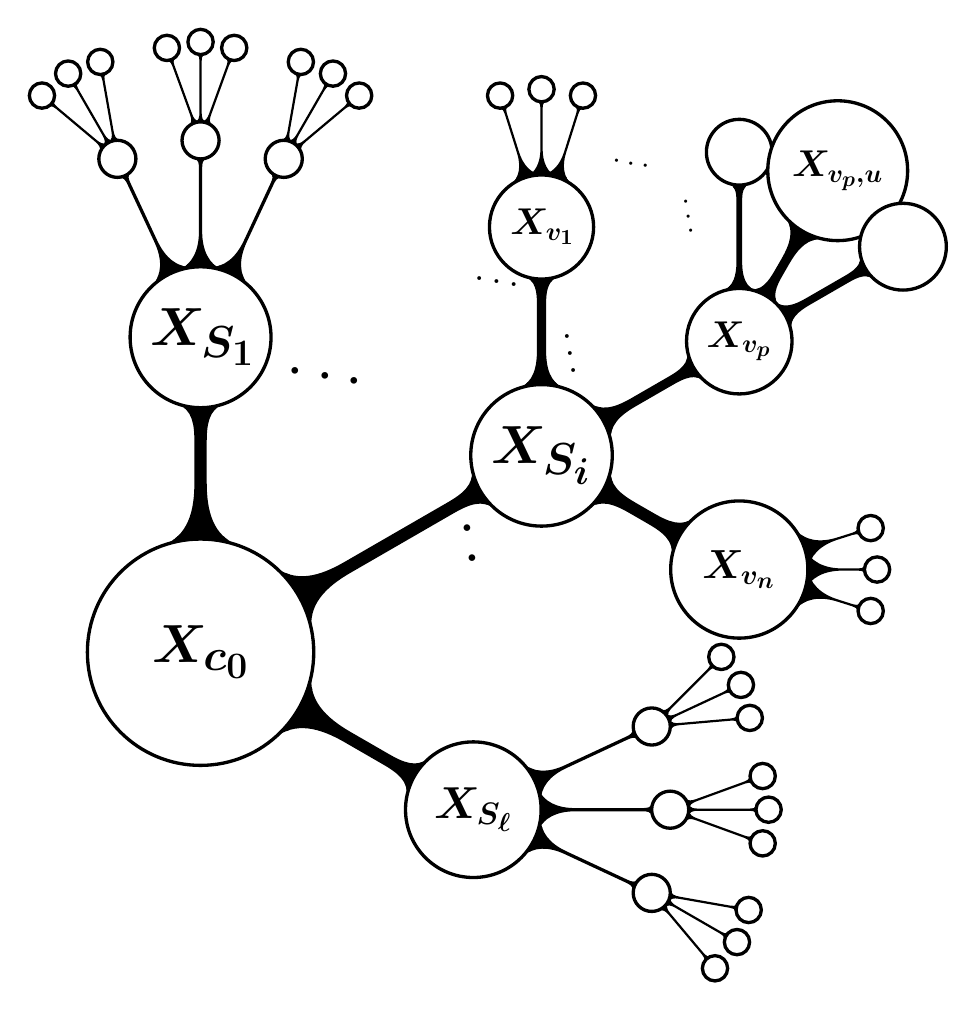
\begin{tikzpicture}


\newcommand{\colorxdb}{black}
\newcommand{\colorxsb}{black}
\newcommand{\colorxvb}{black}
\newcommand{\colorxvub}{black}



  \path[mindmap,concept color=\colorxdb,text=black,]
    node[draw=black,circle,fill=white!50,minimum size=.1cm,scale=0.78] {\Huge $\boldsymbol{X_{c_0}}$}
    [clockwise from=90]
    child[level distance=40mm, concept color=\colorxsb] {
      node[draw=black,circle,fill=white!50,minimum size=.1cm,scale=0.78] {\Huge $\boldsymbol{X_{S_{1}}}$}
      [clockwise from=115]
      child[level distance=25mm,sibling angle=25,concept color=\colorxvb] { node[draw=black,circle,fill=white!50,minimum size=.1cm, scale=0.3] {}
          [clockwise from=140]
          child[level distance=12.5mm,sibling angle=20,concept color=\colorxvub] { node[draw=black,circle,fill=white!50,minimum size=.1cm, scale=0.3] {} }
          child[level distance=12.5mm,sibling angle=20,concept color=\colorxvub] { node[draw=black,circle,fill=white!50,minimum size=.1cm, scale=0.3] {} }
          child[level distance=12.5mm,sibling angle=20,concept color=\colorxvub] { node[draw=black,circle,fill=white!50,minimum size=.1cm, scale=0.3] {} }
      }
      child[level distance=25mm,sibling angle=25, concept color=\colorxvb] { node[draw=black,circle,fill=white!50,minimum size=.1cm, scale=0.3] {}
          [clockwise from=110.]
          child[level distance=12.5mm,sibling angle=20,concept color=\colorxvub] { node[draw=black,circle,fill=white!50,minimum size=.1cm, scale=0.3] {} }
          child[level distance=12.5mm,sibling angle=20,concept color=\colorxvub] { node[draw=black,circle,fill=white!50,minimum size=.1cm, scale=0.3] {} }
          child[level distance=12.5mm,sibling angle=20,concept color=\colorxvub] { node[draw=black,circle,fill=white!50,minimum size=.1cm, scale=0.3] {} }
      }
      child[level distance=25mm,sibling angle=25, concept color=\colorxvb] { node[draw=black,circle,fill=white!50,minimum size=.1cm, scale=0.3] {}
          [clockwise from=80]
          child[level distance=12.5mm,sibling angle=20,concept color=\colorxvub] { node[draw=black,circle,fill=white!50,minimum size=.1cm, scale=0.3] {} }
          child[level distance=12.5mm,sibling angle=20,concept color=\colorxvub] { node[draw=black,circle,fill=white!50,minimum size=.1cm, scale=0.3] {} }
          child[level distance=12.5mm,sibling angle=20,concept color=\colorxvub] { node[draw=black,circle,fill=white!50,minimum size=.1cm, scale=0.3] {} }
      }
    }
    child[concept color=\colorxsb] {
      node[draw=black,circle,fill=white!50,minimum size=.1cm,scale=0.78] {\Huge $\boldsymbol{X_{S_{i}}}$}
      [clockwise from=90]
      child[,concept color=\colorxvb] { node[draw=black,circle,fill=white!50,minimum size=.1cm, scale=0.78] {\LARGE$\boldsymbol{X_{v_{1}}}$} 
          [clockwise from=107.5]
          child[level distance=17.5mm,sibling angle=17.5,concept color=\colorxvub] { node[draw=black,circle,fill=white!50,minimum size=.1cm, scale=0.3] {} }
          child[level distance=17.5mm,sibling angle=17.5,concept color=\colorxvub] { node[draw=black,circle,fill=white!50,minimum size=.1cm, scale=0.3] {} }
          child[level distance=17.5mm,sibling angle=17.5,concept color=\colorxvub] { node[draw=black,circle,fill=white!50,minimum size=.1cm, scale=0.3] {} }
      }
      child[concept color=\colorxvb] {
        node[draw=black,circle,fill=white!50,minimum size=.1cm,scale=0.78, clockwise from=90] {\LARGE $\boldsymbol{X_{v_p}}$}
          [clockwise from=90]
          child[concept color=\colorxvub] { node[draw=black,circle,fill=white!50,minimum size=.1cm, scale=0.78] {} }
          child[level distance=25mm, concept color=\colorxvub] { node[draw=black,circle,fill=white!50,minimum size=.1cm, scale=.78, minimum size = 1.5cm,text width=2.1cm, align=center] {
        \LARGE$\boldsymbol{X_{v_{p},u}}$
          } }
          child[concept color=\colorxvub] { node[draw=black,circle,fill=white!50,minimum size=.1cm, scale=1.03] {} }
    }
      child[,concept color=\colorxvb] {
          node[ draw=black,circle,fill=white!50,minimum size=2.05cm, scale=0.85] {\LARGE $\boldsymbol{X_{v_{n}}} $}
          [clockwise from=17.5]
          child[level distance=17.5mm,sibling angle=17.5,concept color=\colorxvub] { node[draw=black,circle,fill=white!50,minimum size=.1cm, scale=0.3] {} }
          child[level distance=17.5mm,sibling angle=17.5,concept color=\colorxvub] { node[draw=black,circle,fill=white!50,minimum size=.1cm, scale=0.3] {} }
          child[level distance=17.5mm,sibling angle=17.5,concept color=\colorxvub] { node[draw=black,circle,fill=white!50,minimum size=.1cm, scale=0.3] {} }
    }
    }
    child[level distance=40mm, concept color=\colorxsb] {
      node[draw=black,circle,fill=white!50,minimum size=.1cm, scale=0.78] {\huge $\boldsymbol{X_{S_{\ell}}}$}
      [clockwise from=25]
      child[level distance=25mm,sibling angle=25,concept color=\colorxvb] { node[draw=black,circle,fill=white!50,minimum size=.1cm, scale=0.3] {}
          [clockwise from=45]
          child[level distance=12.5mm,sibling angle=20,concept color=\colorxvub] { node[draw=black,circle,fill=white!50,minimum size=.1cm, scale=0.3] {} }
          child[level distance=12.5mm,sibling angle=20,concept color=\colorxvub] { node[draw=black,circle,fill=white!50,minimum size=.1cm, scale=0.3] {} }
          child[level distance=12.5mm,sibling angle=20,concept color=\colorxvub] { node[draw=black,circle,fill=white!50,minimum size=.1cm, scale=0.3] {} }
      }
      child[level distance=25mm,sibling angle=25,concept color=\colorxvb] { node[draw=black,circle,fill=white!50,minimum size=.1cm, scale=0.3] {}
          [clockwise from=20.]
          child[level distance=12.5mm,sibling angle=20,concept color=\colorxvub] { node[draw=black,circle,fill=white!50,minimum size=.1cm, scale=0.3] {} }
          child[level distance=12.5mm,sibling angle=20,concept color=\colorxvub] { node[draw=black,circle,fill=white!50,minimum size=.1cm, scale=0.3] {} }
          child[level distance=12.5mm,sibling angle=20,concept color=\colorxvub] { node[draw=black,circle,fill=white!50,minimum size=.1cm, scale=0.3] {} }
      }
      child[level distance=25mm,sibling angle=25,concept color=\colorxvb] { node[draw=black,circle,fill=white!50,minimum size=.1cm, scale=.3] {}
          [clockwise from=-10]
          child[level distance=12.5mm,sibling angle=20,concept color=\colorxvub] { node[draw=black,circle,fill=white!50,minimum size=.1cm, scale=0.3] {} }
          child[level distance=12.5mm,sibling angle=20,concept color=\colorxvub] { node[draw=black,circle,fill=white!50,minimum size=.1cm, scale=0.3] {} }
          child[level distance=12.5mm,sibling angle=20,concept color=\colorxvub] { node[draw=black,circle,fill=white!50,minimum size=.1cm, scale=0.3] {} }
      }
    };

\node[rotate=-80] at (3.4,1.5) {\Huge$\dots$};
\node[rotate=-10] at (1.65,3.5) {\Huge$\dots$};
\node[rotate=-10] at (3.8,4.7) {\Large$\dots$};
\node[rotate=-80] at (4.7,3.75) {\Large$\dots$};
\node[rotate=-10] at (5.5,6.2) {\large$\dots$};
\node[rotate=-80] at (6.2,5.5) {\large$\dots$};



\end{tikzpicture}
}

\end{minipage}
\end{minipage}}
\caption{A tree decomposition $(\mathcal{X},F)$ of the overall conflict graph constructed from the instance of \WEQUIJIT. Observe that the width of this decomposition is~$|X_v|-1 = 4$.}
\label{fig:tw}
\end{figure}


% lax begin Lax117284.Lemma15
\setcounter{lemma}{14}
\begin{lemma}
\label{lem:15}
\WEQUIJIT\ reduces in polynomial time to
\EQUIJIT, raising the treewidth of the overall conflict
graph by at most~$2$.
\end{lemma}
% lax end
Given~$I$ with~$n$ clients,~$m$ days and parameters~$k_j\le m$: append another~$m$ days and
two clients~$c^-,c^+$ whose identical job, on every new day, occupies a stretch later than
every due date of~$I$ (so it conflicts with nothing of~$I$), and ask for the uniform
parameter~$m$. Each of~$c^-,c^+$ requires~$m$ executions. They conflict on every day, so together
occupy all~$2m$ days, with exactly one of them served each day. Each original client~$j$
is blocked on~$k_j$ of the additional days and can run on the other~$m-k_j$ days.
It can therefore reach the uniform requirement~$m$ exactly when it can be served on
at least~$k_j$ original days. Two
clients add at most two to the treewidth.

% copied from the thesis chapter on fairness (content/fairness/fairness.tex, lines 1204-1351)
\begin{figure}[!hbp]
\centering
\begin{subfigure}{0.8\textwidth}
\begin{center}
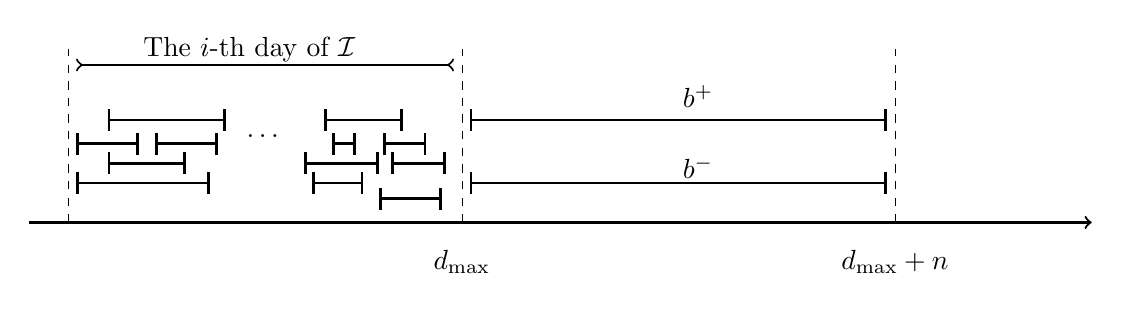
\begin{tikzpicture}

    \def\dmax{5.5}
    \def\eps{.1}
    % main axis
    \draw[thick,->] (0,0) -- (13.5,0) node[anchor=north west] {};
    % I dashed borders
    \draw[line width=0.1, dashed]
    (\dmax,-.) -- (\dmax,2.2) node[anchor=north] {};
    \node at (({\dmax}, -.5) {$d_{\max}$};
    \draw[line width=0.1, dashed]
    (0.5,-.) -- (0.5,2.2) node[anchor=north] {};
    \node at (({11.}, -.5) {$d_{\max}+n$};
    
    \draw[line width=0.1, dashed]
    (11.,-.) -- (11.,2.2) node[anchor=north] {};

    % I
    \draw[line width=.75, >-<]
  ({0.5+\eps}, 2.) -- ({\dmax-\eps}, 2.) node[anchor=north west] {};
  \node at (({\dmax*0.5+\eps*0.5}, 2.2) {The $i$-th day of $\mathcal{I}$};
    
    % I intervals

    \node at (({\dmax*0.5+0.25}, 1.1) {$\dots$};
  \draw[line width=1, |-|]
  ({0.5+\eps}, .5) -- ({2.3}, .5) node[anchor=north west] {};
  \draw[line width=1, |-|]
  ({0.5+\eps}, 1.) -- ({1.5-\eps}, 1.) node[anchor=north west] {};
  \draw[line width=1, |-|]
  ({1.5+\eps}, 1.) -- ({2.5-\eps}, 1.) node[anchor=north west] {};
  \draw[line width=1, |-|]
  (1, .75) -- ({2.}, .75) node[anchor=north west] {};
  \draw[line width=1, |-|]
  (1, 1.3) -- ({2.5}, 1.3) node[anchor=north west] {};
  \draw[line width=1, |-|]
  (1, 1.3) -- ({2.5}, 1.3) node[anchor=north west] {};


\draw[line width=1, |-|]
  (\dmax*0.5+1.7, .3) -- ({\dmax*0.5+2.5}, .3) node[anchor=north west] {};
  \draw[line width=1, |-|]
  ({\dmax*0.5+0.75+\eps}, .5) -- ({\dmax*0.5+1.5}, .5) node[anchor=north west] {};
  \draw[line width=1, |-|]
  ({\dmax*0.5+1.75+\eps}, .75) -- ({\dmax*0.5+2.65-\eps}, .75) node[anchor=north west] {};
  \draw[line width=1, |-|]
  (\dmax*0.5+.75, .75) -- ({\dmax*0.5+1.7}, .75) node[anchor=north west] {};
    \draw[line width=1, |-|]
  ({\dmax*0.5+1.+\eps}, 1.) -- ({\dmax*0.5+1.5-\eps}, 1.) node[anchor=north west] {};
    \draw[line width=1, |-|]
  ({\dmax*0.5+1.65+\eps}, 1.) -- ({\dmax*0.5+2.4-\eps}, 1.) node[anchor=north west] {};
  \draw[line width=1, |-|]
  (\dmax*0.5+1, 1.3) -- ({\dmax*0.5+2.}, 1.3) node[anchor=north west] {};


   \draw[line width=1, |-|]
  (\dmax+\eps, 1.3) -- ({11.-\eps}, 1.3) node[anchor=north west] {};
  \node at (({8.5}, 1.6) {$b^+$};
   \draw[line width=1, |-|]
  (\dmax+\eps, .5) -- ({11.-\eps}, .5) node[anchor=north west] {};
  \node at (({8.5}, .7) {$b^-$};
  
    \end{tikzpicture}
    \caption{When $1\leq i\leq \q$, the jobs of the original clients have the same intervals as in  the $i$-th day of $\mathcal{I}$.}
    \end{center}
    \end{subfigure}

  
% \end{tikzpicture}
 \begin{subfigure}{0.8\textwidth}
        \begin{center}
            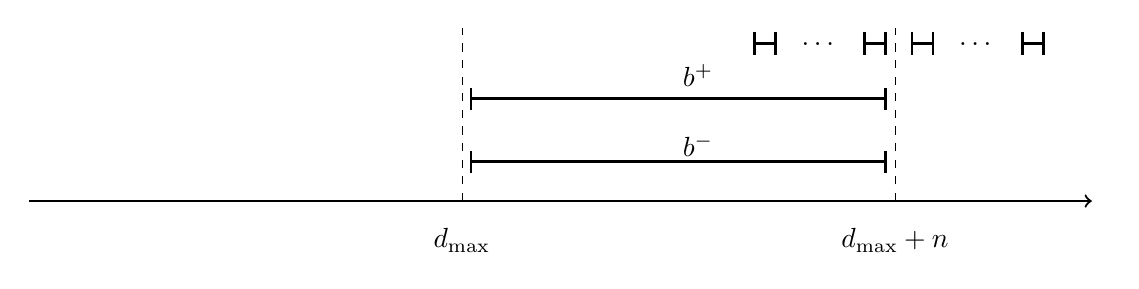
\begin{tikzpicture}

                 \def\dmax{5.5}
    \def\eps{.1}
    % main axis
    \draw[thick,->] (0,0) -- (13.5,0) node[anchor=north west] {};
    % I dashed borders
    \draw[line width=0.1, dashed]
    (\dmax,-.) -- (\dmax,2.2) node[anchor=north] {};
    \node at (({\dmax}, -.5) {$d_{\max}$};
    \node at (({11.}, -.5) {$d_{\max}+n$};
    \draw[line width=0.1, dashed]
    (11.,-.) -- (11.,2.2) node[anchor=north] {};

    
   \draw[line width=1, |-|]
  (\dmax+\eps, 1.3) -- ({11.-\eps}, 1.3) node[anchor=north west] {};
  \node at (({8.5}, 1.6) {$b^+$};
   \draw[line width=1, |-|]
  (\dmax+\eps, .5) -- ({11.-\eps}, .5) node[anchor=north west] {};
  \node at (({8.5}, .7) {$b^-$};


% Intervals over b^- b^+
\foreach \x/\i in
    {
        1/1,2/3,3/1
    }
    {
        \ifthenelse{\i = 0}{
        
        }{
         \ifthenelse{\i = 1}{
                \draw[line width=1, |-|]
                  (\dmax+3+\x*0.7, 2) -- ({\dmax+3+\x*0.7+0.3}, 2) node[anchor=north west] {};
         }{

            \node at (\dmax+3+\x*0.7+0.15, 2) {$\dots$};
         
         }
        }

    }  

% Intervals after b^- b^+
\foreach \x/\i in
    {
        1/1,2/3,3/1
    }
    {
        \ifthenelse{\i = 0}{
        
        }{
         \ifthenelse{\i = 1}{
                \draw[line width=1, |-|]
                  (10.5+\x*0.7, 2) -- ({10.5+\x*0.7+0.3}, 2) node[anchor=north west] {};
         }{

            \node at (10.5+\x*0.7+0.15, 2) {$\dots$};
         
         }
        }

    }  
    
   
\end{tikzpicture}
\caption{When $\q< i\leq2\q$ let the jobs of original clients either intersect the jobs of both $b^-$ and $b^+$  (for $\{\ c\ |\ i-\q \leq k_c\ \}$) \textit{or} intersect no jobs at all (for $\{\ c\ |\ i-\q > k_c\ \}$).}
\end{center}
\end{subfigure}
\caption{An intersection model of the $i$-th day's jobs.}
\label{fig:reduction-unweighted}
\end{figure}


Combining \Cref{lem:14,lem:15} gives \Cref{thm:4a}, since~$4+2=6$.

\subsection{Finding Nice Tree Decompositions}

The dynamic programs below consume \emph{nice} tree decompositions, whose nodes are leaves,
\emph{introduce} nodes that add one vertex to the bag of their child, \emph{forget} nodes that
remove one, and \emph{join} nodes with two children of equal bag.
% lax begin lax-689794
For the word RAM, a graph on~$n$ vertices is the word~$n$ followed by its adjacency matrix row
by row, and a nice decomposition is a word of~$N$ records, one per node, listing its kind, its
vertex and its second child, each node after its children; the bags are determined from the
leaves upward.

\begin{supportingtheorem}[Bodlaender and Kloks]
Given a graph and a nice tree decomposition of width at most~$\ell$, one can decide whether
the treewidth is at most~$k$ and, if so, find a nice decomposition of width at most~$k$, in
time~$2^{\bigO(\ell^3)}\cdot\mathrm{poly}$.
\end{supportingtheorem}

\begin{supportingtheorem}[Bodlaender]
Given a graph and~$k$, one can decide whether the treewidth is at most~$k$ and, if so, find a
nice decomposition of width at most~$k$, in time~$2^{\bigO(k^3)}\cdot\mathrm{poly}$.
\end{supportingtheorem}
Bodlaender's theorem is formalized with an algorithm that is done slightly differently than
in the paper: the exact dynamic program of Bodlaender and Kloks over \emph{characteristics} of
partial decompositions, applied vertex by vertex. A decomposition of the first~$i$ vertices
is extended to one of the first~$i+1$ by inserting the new vertex into every bag, which raises
the width by one, and the improvement step of the previous theorem brings the width back down.
Its running time is proved on a verified virtual machine for a functional language, whose
runs are transferred to the word RAM, and is polynomial in the length of the word times~$2^{\bigO(k^3)}$. The statement used for \Cref{thm:4b} is its case for the overall conflict
graph of an instance, obtained from the proved theorem of the registered submission lax-689794 (\emph{Finding Tree Decompositions of Small Treewidth}).
% lax end

\subsection{Fixed-Parameter Tractability}

% lax begin Lax117284Proofs.TreewidthReal.fpt_byDaysAndTreewidth
\setcounter{theorem}{3}
\begin{theorem}[Days and Treewidth]
\label{thm:4b}
\EQUIJIT\ is fixed-parameter tractable with respect to~$m+\tau$.
\end{theorem}
% lax end
A dynamic program over a nice tree decomposition records the schedules on each bag
that extend to feasible, fair schedules on the clients in its subtree. A state specifies,
for each day, which clients of the bag are served. The transitions combine these
restrictions at introduce, forget and join nodes. The verified implementation establishes
fixed-parameter tractability; no sharper running-time bound is asserted here.

% lax begin Lax117284Proofs.Theorem4Clients.fpt_byClients
\setcounter{theorem}{3}
\begin{theorem}[Number of Clients]
\label{thm:4c}
\EQUIJIT\ is fixed-parameter tractable with respect to the number~$n$ of clients.
\end{theorem}
% lax end
% lax begin Lax117284.IlpClients
The reduction groups days by their conflict relation. The formal construction reserves~$2^{n^2}$ relation types and~$2^n$ subsets of clients, giving exactly~$2^{n^2+n}+n$ variables, including one slack variable per client, and~$2^{n^2}+n$
constraints. The constraint matrix depends only on~$n$; the right-hand sides record
counts of day types and the allowed number of rejections.

The source uses fixed-dimension integer programming~\cite{Lenstra83}. The formalization
instead proves an algorithm for this particular family. It enumerates certificates in a
finite search space whose size depends only on~$n$, reconstructs candidate solutions
from each certificate and the right-hand sides, and checks the constraints. The
normalization and certificate-completeness lemmas justify this search. This establishes
fixed-parameter tractability without enumerating every assignment up to the right-hand
sides. The scheduling decision program separately handles short inputs by enumeration.
% lax end

\section{Formalization Notes}

Running-time bounds are verified for word RAM programs compiled through the archive's
IMP+ compiler (\texttt{lax-808846}). The submission includes proofs of its 2-SAT
and bipartite matching algorithms, and of the algorithm of Bodlaender and Kloks for finding
nice tree decompositions of small width. It uses Tovey's bounded-occurrence satisfiability theorem
(\texttt{lax-345332}), interval scheduling with eligible machine sets
(\texttt{lax-888481}), and the Hitting Set hardness of just-in-time scheduling in
flexible flow shops (\texttt{lax-496464}). The hardness arguments also use the archive's Cook--Levin
theorem and CNF encoding (\texttt{lax-429075}) and the equivalence of word RAM
and Turing-machine polynomial time (\texttt{lax-759944}). The concept pages and
proof network specify the hypotheses and dependencies of each result.

\section{Discussion}

The formalization adjusts the placement of inactive jobs to preserve the conflict
graph required by the treewidth argument. A dummy interval blocks the inactive jobs,
which occupy separate, disjoint slots within it. The development also supplies the
NP-hardness proof for the regular \MCIS\ instances used by the construction.
The concept pages describe these details and the resulting tree decomposition.

\begin{thebibliography}{9}
\bibitem{HHIMS}
K.~Heeger, D.~Hermelin, Y.~Itzhaki, H.~Molter and D.~Shabtay.
\newblock Fair Repetitive Interval Scheduling.
\newblock \emph{Algorithmica}, 2025.
\newblock \doi{10.1007/s00453-025-01322-y}

\bibitem{Sung05}
S.~C. Sung and M.~Vlach.
\newblock Maximizing Weighted Number of Just-in-Time Jobs on Unrelated Parallel Machines.
\newblock \emph{Journal of Scheduling} 8(5):453--460, 2005.
\newblock \doi{10.1007/s10951-005-2860-z}

\bibitem{Tovey84}
C.~A. Tovey.
\newblock A Simplified NP-Complete Satisfiability Problem.
\newblock \emph{Discrete Applied Mathematics} 8(1):85--89, 1984.
\newblock \doi{10.1016/0166-218X(84)90081-7}

\bibitem{Lenstra83}
H.~W. Lenstra, Jr.
\newblock Integer Programming with a Fixed Number of Variables.
\newblock \emph{Mathematics of Operations Research} 8(4):538--548, 1983.
\newblock \doi{10.1287/moor.8.4.538}
\end{thebibliography}

\end{document}
